\documentclass{article}

\usepackage{graphicx}
\usepackage{tikz}
\usepackage{tikzsymbols}
\usetikzlibrary{calc,patterns,shapes.geometric}
\pagestyle{empty}
\usepackage[margin=0pt]{geometry}
\geometry{papersize={14in,12in}}

\def\centerarc[#1](#2)(#3:#4:#5){\draw[#1] ($(#2)+({#5*cos(#3)},{#5*sin(#3)})$) arc (#3:#4:#5);}

\begin{document}
	\begin{figure}
		\centering
		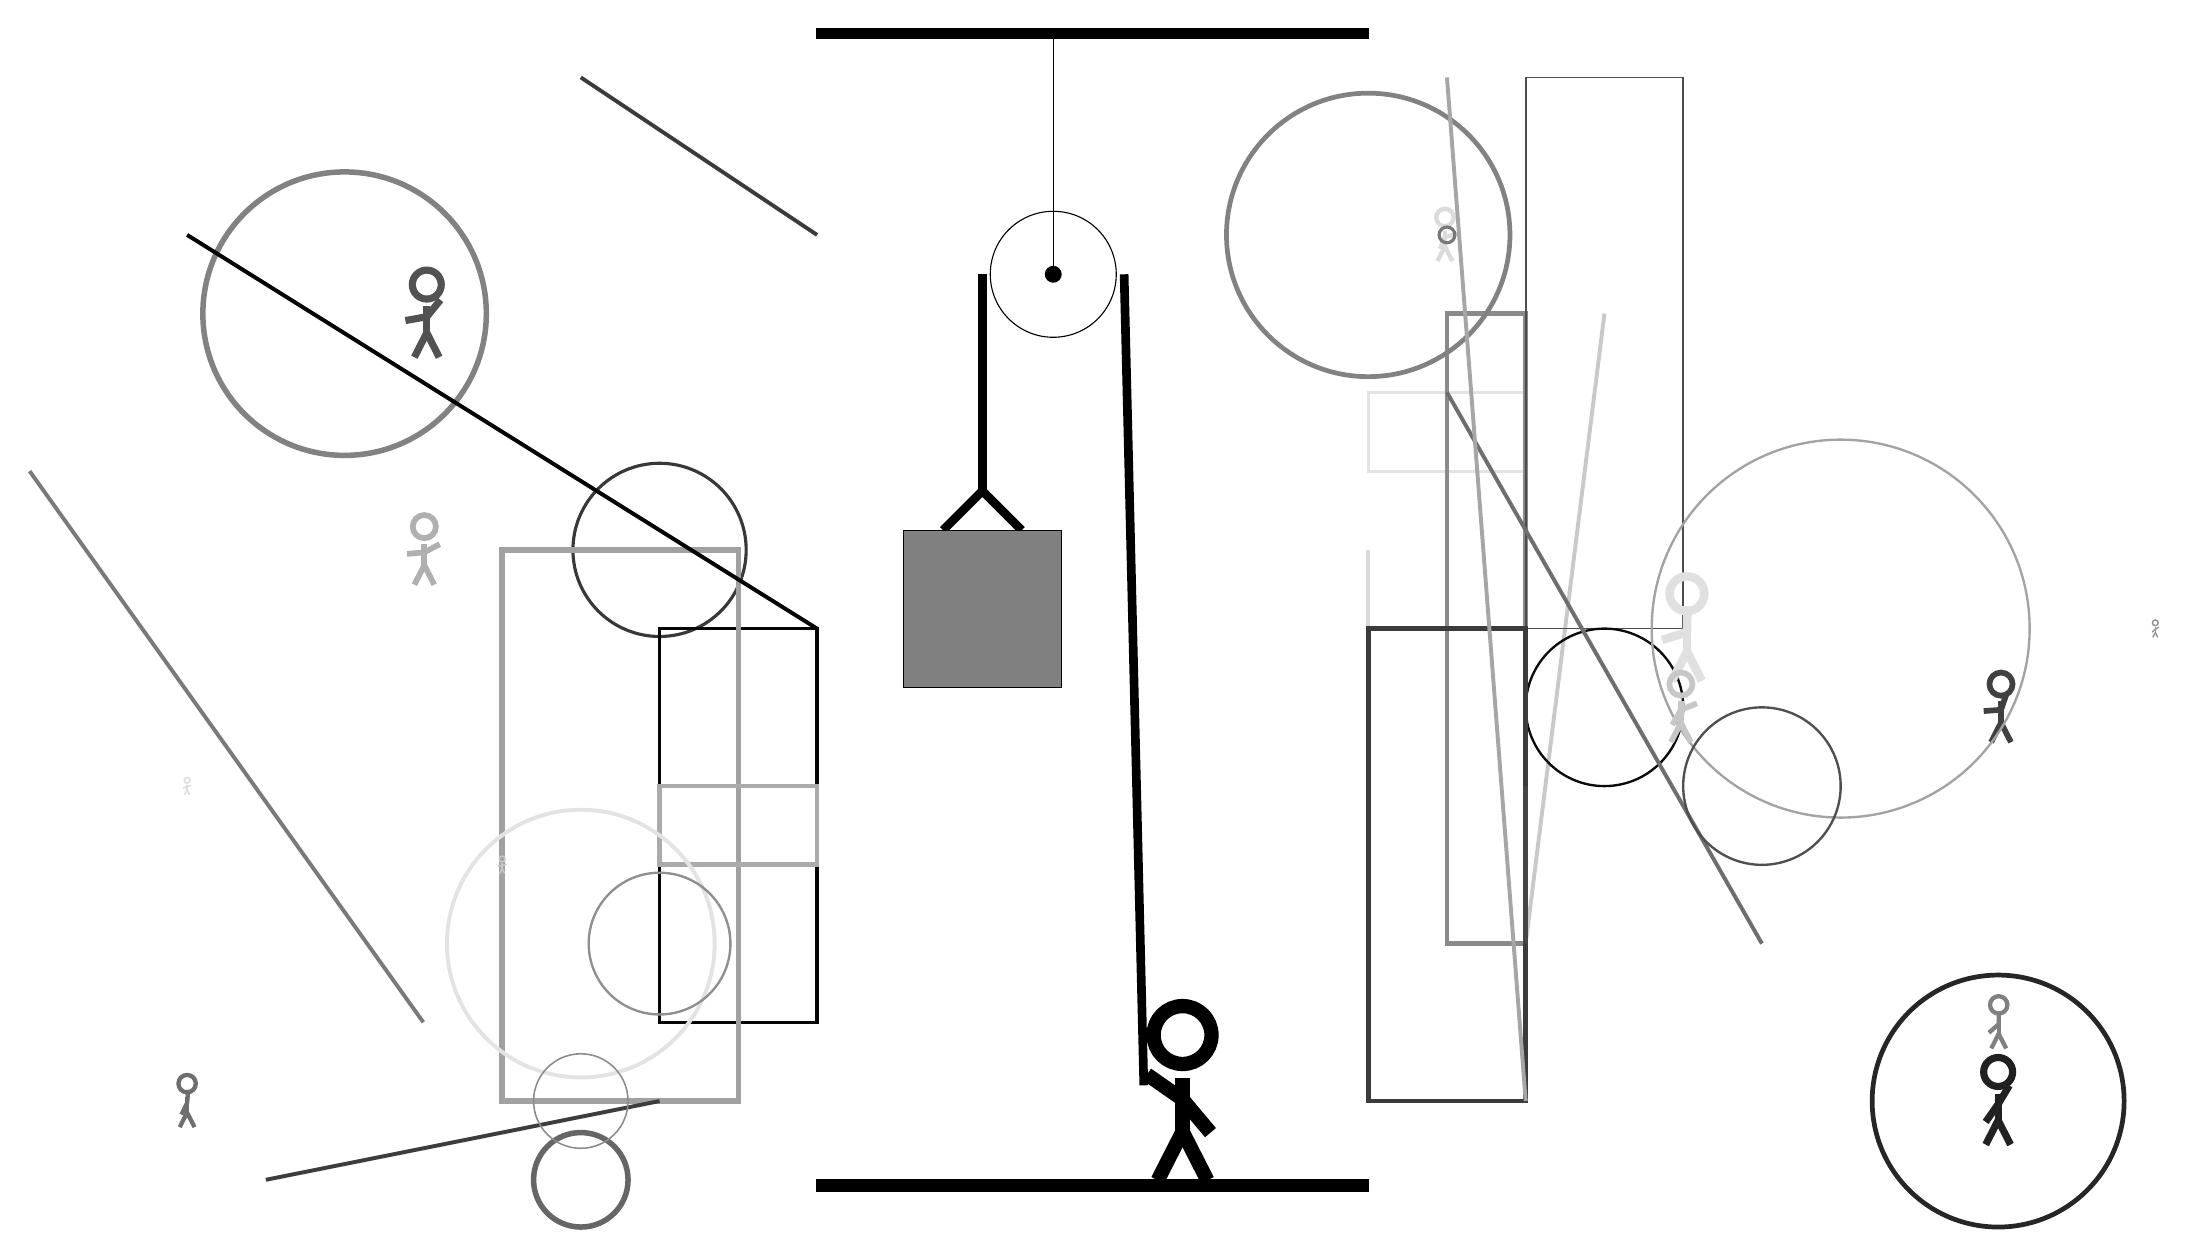
\begin{tikzpicture}
			%%%%% START %%%%%
			
			\draw[fill=black] (-2, 11.5) rectangle (5, 11.625);
			
			\draw (1, 8.5) circle (0.8);
			\draw[fill=black] (1, 8.5) circle (0.1);
			\draw (1, 11.5) -- (1, 8.5);
			
			\draw[line width=1.1mm] (-0.4, 5.25) -- (0.1, 5.75) -- (0.6, 5.25);
			\draw[fill=black!50] (-0.9, 5.25) rectangle (1.1, 3.25);
			
			\draw[line width=1.1mm] (0.1, 8.5) -- (0.1, 5.75);
			\centerarc[line width=1.1mm](1, 8.5)(0:180:0.9);
			\draw[line width=1.1mm](1.9, 8.5) -- (2.15, -1.8);
			
			\node at (2.6, -1.9) {\Strichmaxerl[10][-35][-50]};
			
			\draw[line width=0.4mm, color=black!11] (5, 7) rectangle (7, 6);
			
			\draw[line width=0.5mm, color=black!77](-5, 11) -- (-2, 9);
			\draw [line width=0.4mm, color=black!78](-4, 5) circle (1.1);
			\draw[line width=0.4mm, color=black!98] (-4, -1) rectangle (-2, 4);
			\draw[line width=0.5mm, color=black!21](7, 0) -- (8, 8);
			
			\draw[line width=0.5mm, color=black!76](5, 3) -- (5, -2);
			
			\node[line width=0.7mm, color=black!14] at (6, 9) {\Strichmaxerl[3][67][13]};
			\draw[line width=0.6mm, color=black!46] (7, 8) rectangle (6, 0);
			\draw [line width=0.6mm, color=black!85](13, -2) circle (1.6);
			\draw[line width=0.7mm, color=black!37] (-3, -2) rectangle (-6, 5);
			\node[line width=0.3mm, color=black!75] at (13, 3) {\Strichmaxerl[4][4][71]};
			\draw[line width=0.2mm, color=black!70] (7, 11) rectangle (9, 4);
			\draw [line width=0.7mm, color=black!49](-8, 8) circle (1.8);
			
			\draw [line width=0.6mm, color=black!49](5, 9) circle (1.8);
			\draw[line width=0.5mm, color=black!15](5, 2) -- (5, 5);
			\node[line width=0.2mm, color=black!14] at (-10, 2) {\Strichmaxerl[1][17][15]};
			\node[line width=0.3mm, color=black!87] at (13, -2) {\Strichmaxerl[5][55][59]};
			
			\draw [line width=0.3mm, color=black!96](8, 3) circle (1.0);
			\node[line width=0.5mm, color=black!12] at (9, 4) {\Strichmaxerl[6][17][89]};
			
			\node[line width=0.7mm, color=black!50] at (13, -1) {\Strichmaxerl[3][41][89]};
			\node[line width=0.5mm, color=black!43] at (15, 4) {\Strichmaxerl[1][42][29]};
			
			\draw[line width=0.6mm, color=black!77] (5, -2) rectangle (7, 4);
			\draw [line width=0.3mm, color=black!36](11, 4) circle (2.4);
			\node[line width=0.6mm, color=black!31] at (-7, 5) {\Strichmaxerl[4][5][28]};
			\draw [line width=0.7mm, color=black!60](-5, -3) circle (0.6);
			\draw[line width=0.6mm, color=black!73] (7, 0) rectangle (7, 2);
			\draw [line width=0.4mm, color=black!53](6, 9) circle (0.1);
			\draw[line width=0.6mm, color=black!33] (-2, 2) rectangle (-4, 1);
			
			\draw[line width=0.5mm, color=black!57](6, 7) -- (10, 0);
			\draw [line width=0.5mm, color=black!11](-5, 0) circle (1.7);
			\draw [line width=0.3mm, color=black!44](-4, 0) circle (0.9);
			
			\draw[line width=0.5mm, color=black!76](-4, -2) -- (-9, -3);
			\node[line width=0.2mm, color=black!68] at (-7, 8) {\Strichmaxerl[5][10][51]};
			\draw[line width=0.5mm, color=black!52](-7, -1) -- (-12, 6);
			
			\node[line width=0.2mm, color=black!22] at (-6, 1) {\Strichmaxerl[1][7][20]};
			\node[line width=0.2mm, color=black!22] at (9, 3) {\Strichmaxerl[4][60][22]};
			
			\draw [line width=0.3mm, color=black!69](10, 2) circle (1.0);
			\draw[line width=0.5mm, color=black!35](6, 11) -- (7, -2);
			\node[line width=0.4mm, color=black!57] at (-10, -2) {\Strichmaxerl[3][64][85]};
			\draw[line width=0.5mm, color=black!99](-2, 4) -- (-10, 9);
			
			\draw [line width=0.2mm, color=black!45](-5, -2) circle (0.6);
			
			
			\draw[fill=black] (-2, -3) rectangle (5, -3.15);
			
			%%%%% END %%%%%
		\end{tikzpicture}
	\end{figure}	
\end{document}